\problemname{\problemyamlname}

\begin{wrapfigure}{r}{5.5cm}
    \centering
    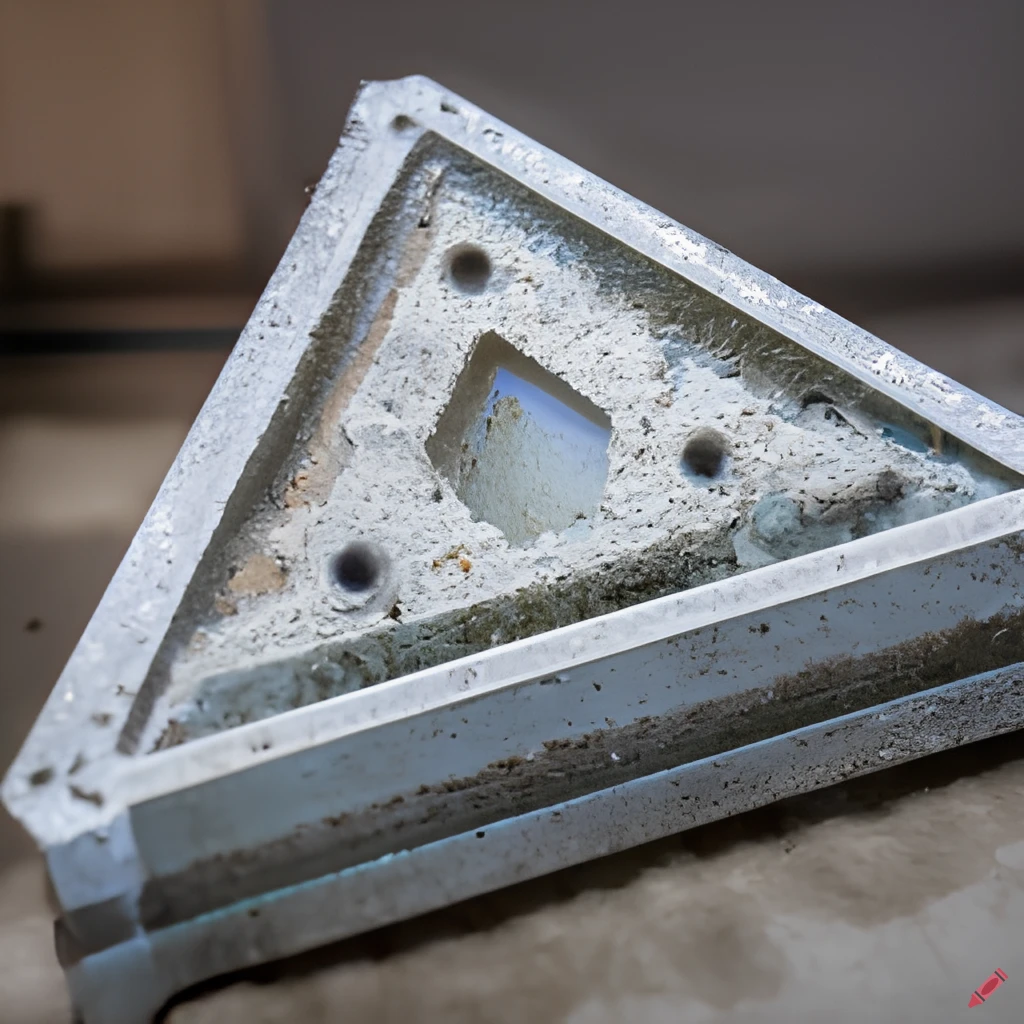
\includegraphics[width=5.5cm]{palindromium.jpg}
\end{wrapfigure}
Un débat a éclaté entre les étudiants de l'UMons et de l'UCLouvain.
Ils ne parviennent pas à se mettre d'accord sur la meilleure des deux universités, surtout dans le domaine scientifique.
Nous avons besoin de votre aide pour les départager et ainsi avantager votre université au sujet d'un tout nouveau métal appelé ``palindronium''.

Votre mission est d'optimiser la production de palindronium dans votre université, production pour l'instant très coûteuse.
Pour l'optimiser, le métal doit être fabriqué dans un moule d'une forme d'un triangle rectangle dont la longueur de l'hypoténuse est un nombre entier et un palindrome.
Par souci d'espace, vous ne pouvez modéliser qu'un seul moule, et celui-ci doit pouvoir rentrer dans un carré de taille $n \times n$, il doit ainsi avoir une aire maximale.

Un nombre est un palindrome s'il ne change pas lorsqu'il est lu de gauche à droite ou de droite à gauche, chiffre par chiffre.
Par exemple, $191$ est un palindrome, mais $155$ ne l'est pas.
Votre but est d'avoir la plus grande aire possible sous ces contraintes ! Attention cependant, on ne demande qu'à l'hypoténuse d'être entier et d'être un palindrome, les autres côtés n'ont aucune restriction.

Par exemple, si le carré dans lequel votre moule doit rentrer a une taille de $12 \times 12$, vous pouvez fabriquer un moule de taille $(3,4,5)$ car $5$, l'hypothénuse, est un palindrome, ce qui donnera une aire de moule de $6$. Vous pouvez aussi faire un moule de taille $(\sqrt{105},4,11)$.

\begin{figure}[h]
\centering
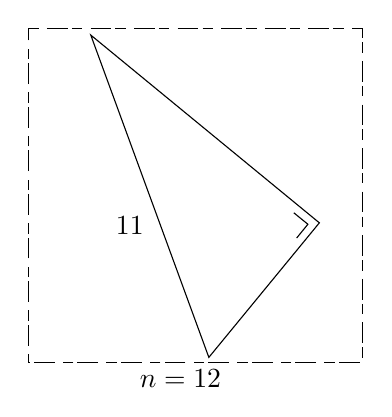
\begin{tikzpicture}[x=0.75pt,y=0.75pt,yscale=-1,xscale=1]
%uncomment if require: \path (0,300); %set diagram left start at 0, and has height of 300

%Shape: Rectangle [id:dp8053011662910811]
\draw  [dash pattern={on 3.75pt off 3pt on 7.5pt off 1.5pt}] (219.5,49.5) -- (380.75,49.5) -- (380.75,210.7) -- (219.5,210.7) -- cycle ;
%Shape: Right Triangle [id:dp47291251588999583]
\draw   (306.52,208.08) -- (249.63,52.79) -- (359.76,143.26) -- cycle ;
%Shape: Right Angle [id:dp6371826673456693]
\draw   (347.44,138.41) -- (354.24,143.94) -- (348.83,150.58) ;

% Text Node
\draw (260.5,139) node [anchor=north west][inner sep=0.75pt]   [align=left] {$\displaystyle 11$};
% Text Node
\draw (272,212.5) node [anchor=north west][inner sep=0.75pt]   [align=left] {$\displaystyle n=12$};
\end{tikzpicture}
\end{figure}

\begin{Input}
	Un entier $n$ ($1 \le n \le 10^8$) donnant la longueur des côtés du carré devant contenir le moule triangulaire.
\end{Input}

\begin{Output}
	Une ligne contenant l'aire maximale que vous pouvez obtenir avec un
	moule, à une erreur absolue ou relative de maximum $10^{-6}$.
\end{Output}
